\twocolumn[
\begin{center}
\title{\color[cmyk]{1, 0.57, 0, 0.38}{\Huge\bfseries Fedora Project\\}} % definisco il titolo dell'articolo
\author{\scriptsize Gabriele Trombini (mailga@fedoraonline.it)} % definisco l'autore e altre informazioni
\date{}
\end{center}
{\color[cmyk]{1, 0.46, 0, 0}\LARGE Il Fedora Project - comprensione di un grande fenomeno legato al software libero}\\
\maketitle
\normalsize
\doublespacing
\hfill
]
\lettrine[lines=1, loversize=0.1, lraise=0.1]{\color[cmyk]{0.5, 0, 1, 0}\bfseries C}{}redo che tutti noi ci siamo chiesti almeno una volta quale lavoro stava dietro al nostro sistema operativo. Quali fossero i mezzi utilizzati e quante persone erano impegnate nel suo sviluppo.\\

Tutto è riconducibile al Fedora Project {\itshape (http://fedoraproject.org/)} che si può definire un contenitore per le idee che vengono portate avanti da singoli utenti che condividono il proprio lavoro.\\

\begin{figure}[htbp]
\centering
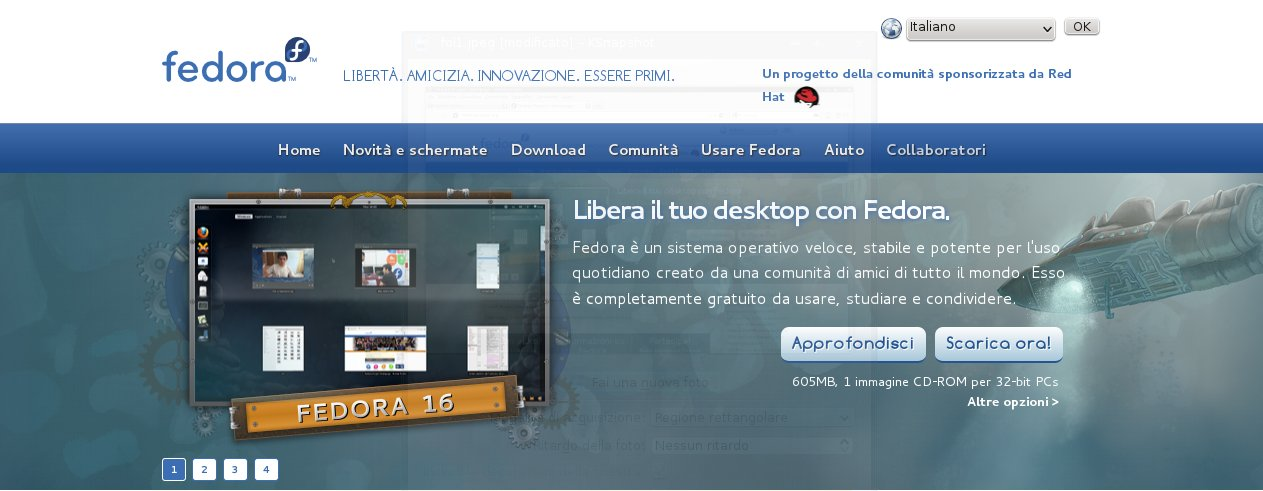
\includegraphics[scale=.20]{articoli/varie/immagini/fp.jpeg}
\caption{Il sito del Fedora Project\label{Fig.1: Fedora Project}}
\end{figure}

Chiunque voglia impegnarsi attivamente nel progetto potrebbe trovare un po' difficoltoso avventurarsi all'interno del suo sito web in quanto la sua organizzazione è molto capillare.\\

Vediamo, in questo articolo, di chiarire un po' le idee degli utenti.\\

Innanzi tutto è bene precisare i termini del legame tra Red Hat ed il Fedora Project, come spiegato all'indirizzo web {\itshape http://it.redhat.com/resourcelibrary/arti cles/relationship-between-fedora-and-\\ rhel}, dove ben si definisce che sono due entità separate, la prima con l'obiettivo dell'IT, la seconda a vantaggio della comunità:\\
{\itshape ``Le dimensioni e l'esperienza della comunità di Fedora, rendono Fedora l'incubatrice e il terreno di prova ideale per le funzioni che, in seguito, verranno integrate in Red Hat Enterprise Linux. Per soddisfare i requisiti di qualità e affidabilità che rendono Red Hat Enterprise Linux la scelta ideale per le applicazioni di importanza cruciale, i test e processi di controllo di qualità di Red Hat Enterprise Linux sono separati e distinti da quelli di Fedora.\\

Fedora: sviluppo rapido della tecnologia più recente.\\

La comunità di Fedora è composta da migliaia di utenti, collaboratori e sostenitori, i quali interagiscono tramite i forum online, le mailing list ed i wiki per sostenersi l'un l'altro. Con uno sviluppo e un ciclo di distribuzione molto rapidi, Fedora fornisce la tecnologia più recente sulle piattaforme hardware attuali.\\

Red Hat Enterprise Linux: piattaforma open source stabile e supportata.\\

Se si sceglie di eseguire Red Hat Enterprise Linux, si entra in stretto contatto con il principale fornitore di soluzioni open source. Non solo si ottiene una piattaforma affidabile e stabile, con un ciclo di vita di 10 anni, ma si può godere anche dei vantaggi offerti da organizzazioni internazionali di progettazione, consulenza e assistenza. Una sottoscrizione Red Hat Enterprise garantisce l'accesso a software e manutenzione di alta qualità, oltre alle informazioni e all'assistenza che si estendono al ciclo di vita e all'architettura dell'intera infrastruttura.''} \\

Nella pagina del sito Fedora {\itshape http://fedo raproject.org/sponsors} si specifica che la casa madre mette a disposizione del progetto infrastrutture, personale e finanziamenti:\\
{\itshape ``Red Hat, Inc. è lo sponsor principale per il Fedora Project. Red Hat fornisce al Fedora project una varietà di risorse, che includono il supporto dei dipendenti a tempo pieno, infrastrutture hardware e di banda, finanziamento degli eventi e consulenza legale.''}\\

Ricordiamoci bene, però, che Red Hat non è Fedora.\\

Il Fedora Project è il contenitore ideale dove, chiunque di noi, può sostenere, integrare,
migliorare, creare i progetti che diventeranno parte integrante dell'idea che
sta alla base di tutto questo.\\


Non è possibile scindere la totalità del progetto dal sistema operativo perchè
esso è l'emanazione ultima di quello che è stato creato; la sua punta di
diamante.\\

Prima di essere un sistema operativo, Fedora è un crocevia di libero pensiero.
E' riduttivo, infatti, qualificare il Fedora Project come un sistema operativo;
alle spalle di esso c'è una comunità internazionale che sostiene i settori di
sviluppo.\\

Le attività del progetto son molteplici, dallo sviluppo di applicazioni, allo
sviluppo di rami del kernel, da quello del design a quello della
internazionalizzazione, da quello del marketing a quello del web e altro ancora.\\

La distanza tra l'utilizzatore ed il progetto, non è poi così lontana, anzi, è a
portata di mano! Una semplice digitazione di {\itshape www.fedoraproject.org} sulla barra degli
indirizzi e si è già dentro, immersi nelle possibilità che ti può
dare.\\
I valori alla base del lavoro di tutte le persone coinvolte, sono quattro:
\begin{itemize}
\item 
\includegraphics[scale=.20]{articoli/varie/immagini/4f-freedom.png} libertà 
\item 
\includegraphics[scale=.20]{articoli/varie/immagini/4f-friends.png} comunità
\item 
\includegraphics[scale=.20]{articoli/varie/immagini/4f-features.png} condivisione
\item 
\includegraphics[scale=.20]{articoli/varie/immagini/4f-first.png} innovazione
\end{itemize}
e ciascun contributo deve rispettare questi valori.\\

In questo articolo vorrei soffermarmi sul concetto di comunità, estesa al mondo intero, entro la quale ciascuno di noi può (come detto) dare il proprio contributo.\\

I mezzi a disposizione degli utenti sono davvero molti e molto potenti, a cominciare proprio da una area di interesse ben definita.\\

Dividiamo pure in macroaree all'interno delle quali è possibile trovare il proprio spazio specifico e ben dettagliato:
\begin{itemize}
\item 
\includegraphics[scale=.20]{articoli/varie/immagini/join-writer.png} redattore 
\item 
\includegraphics[scale=.20]{articoli/varie/immagini/join-designer.png} disegnatore
\item 
\includegraphics[scale=.20]{articoli/varie/immagini/join-people.png} comunicatore
\item 
\includegraphics[scale=.20]{articoli/varie/immagini/join-osdevel.png} sviluppatore del sistema operativo
\item 
\includegraphics[scale=.20]{articoli/varie/immagini/join-translator.png} traduttore
\item 
\includegraphics[scale=.20]{articoli/varie/immagini/join-webdevel.png} sviluppatore web o amministratore
\end{itemize}
Prima di andare ad analizzare questi ruoli, è bene specificare il ruolo del FAS (Fedora Account System), a cui ci si deve iscrivere, per poter iniziare la propria attività in favore di Fedora.\\

Il FAS, raggiungibile all'indirizzo {\itshape https:// admin.fedoraproject.org/accounts/user/ new} è il sistema per poter richiedere l'associazione ad un gruppo, gestito dagli amministratori. Infatti gli iscritti sono tutti gli appartenenti ai gruppi di lavoro ed è all'interno di esso che è possibile sottoscrivere la domanda di ammissione.\\

Avere un account FAS valido ci permette di avere uno spazio personale nel wiki all'interno del quale è possibile descrivere le proprie esperienze ed i propri contributi. \\
\begin{figure}[htbp]
\centering
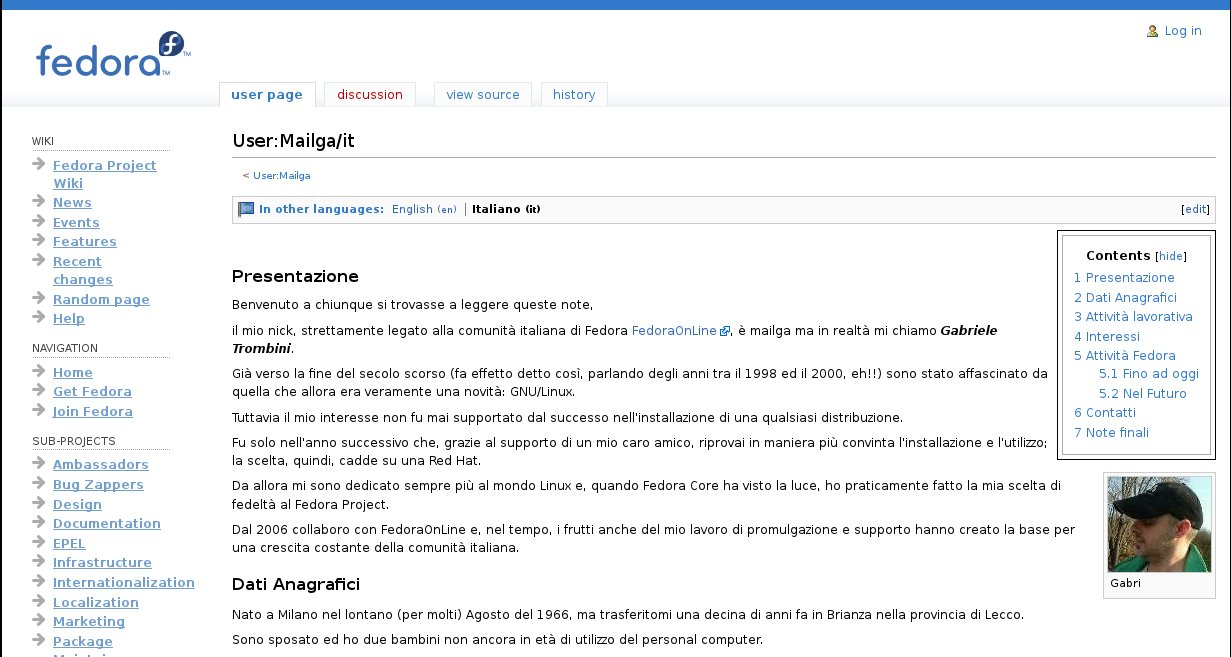
\includegraphics[scale=.20]{articoli/varie/immagini/mailga-wiki.jpeg}
\caption{pagina wiki Mailga\label{Fig.1: server git}}
\end{figure}

Nella pagina web {\itshape https://fedoraproject. org/wiki/Projects} è possibile avere una lista dettagliata e le spiegazioni dei vari progetti.\\

\begin{figure}[!h]
\centering
{\bfseries Redattore 
\includegraphics[scale=.30]{articoli/varie/immagini/join-writer.png}}
\end{figure}
Il ruolo di redattore è particolarmente adatto a coloro che hanno particolare facilità di scrittura. In questa area trovano spazio sia i collaboratori che scrivono i contributi, sia coloro che li traducono nelle varie lingue.\\

\begin{figure}[!hp]
\centering
{\bfseries Disegnatore 
\includegraphics[scale=.30]{articoli/varie/immagini/join-designer.png}}
\end{figure}
In questo gruppo potrà trovare una attività congeniale chi è particolarmente abile nelle arti grafiche.\\

\begin{figure}[!h]
\centering
{\bfseries Comunicatore 
\includegraphics[scale=.30]{articoli/varie/immagini/join-people.png}}
\end{figure}
Questa macrosezione è pensata per le persone che hanno attitudini alla comunicazione, sia essa in pubblico che attraverso attività di marketing.\\

\begin{figure}[!h]
\centering
{\bfseries Sviluppatore sistema operativo 
\includegraphics[scale=.30]{articoli/varie/immagini/join-osdevel.png}}
\end{figure}
I gruppi appartenenti a questa categoria sono fondamentali per la riuscita del sistema operativo. Le persone con conoscenze sulla programmazione potrebbero partecipare alle attività degli sviluppatori.\\

\begin{figure}[!h]
\centering
{\bfseries Traduttore 
\includegraphics[scale=.30]{articoli/varie/immagini/join-translator.png}}
\end{figure}
Un'altra sezione veramente importante per la diffusione del sistema nei vari paesi del mondo è proprio questa. Chiunque possa aiutare nella traduzione di tutta la documentazione Fedora nella propria lingua madre, avendo conoscenze dell'inglese, troverà ampio spazio.\\

\begin{figure}[!h]
\centering
{\bfseries Sviluppatore web/sysadmin 
\includegraphics[scale=.30]{articoli/varie/immagini/join-webdevel.png}}
\end{figure}
Infine, chi è addentro al linguaggio web, allo sviluppo di applicazioni web e/o all'amministrazione dei sistemi Linux può davvero risultare fondamentale per l'infrastruttura del Fedora Project.\\

Tutto quanto gira intorno e all'interno del progetto è nato nello spirito open e free, che abbiamo visto essere tra i fondamenti delle attività ad esso legate.\\

Ed è proprio in questo che si deve partire per comprendere il fenomeno, perchè chi non intende lasciare libera una comunità di proporre, di decidere e anche di sbagliare, non potrà sperare di ottenere risultati apprezzabili.\\
